\section{Grundlagen}
Im Sinne eines Hochregallager besteht eine Gasse aus einer rechten und einer linken Regalwand während sich in der Mitte der beiden Wände ein Korridor für das Regalbediengerät befindet. Die Regalwände sind in Lagerplätze unterteilt, die von Regalbediengerät be- und entladen werden. Hochregallager können aus einer beliebigen Anzahl Gassen bestehen. Im Normalfall befindet sich an einer Stirnseite der Gassen die sogenannte Vorzone, welche die Aufgabe hat, die Lagergüter auf die zugeweisen Gassen zu verteilen. 
%
\begin{figure}[H]
  \begin{center}
    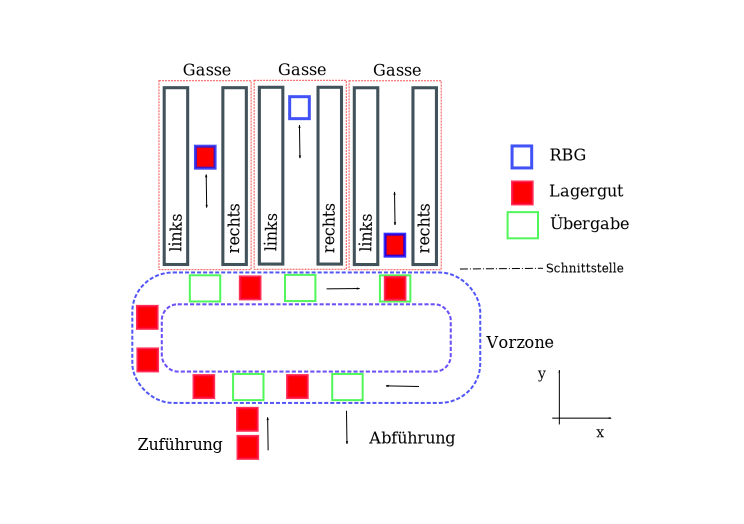
\includegraphics[width=0.8\textwidth]{images/uebersicht.png}
    \caption{Übersicht}
    \label{fig:overview}
  \end{center}
\end{figure}
%

%
\subsection{Allgemeine Grundlagen}

%
\begin{table}[H]
  \caption{Benennungen}
  \label{tab:desc}

  \begin{center}
    \begin{tabular}{cc}
       Location & Lager\\
       Gap & Gasse\\
       Grid & Regalwand \\
       Column & Spalten im Regal \\
       Row & Zeilen im Regal \\
       Bin & Lagerfach \\
       Rack feeder & Regelbediengerät \\
    \end{tabular}
  \end{center}
\end{table}
%

\subsubsection{Koordinaten}
Der Koordinatenursprung befinet sich in der linken unteren Ecke der Regalwand (Grid). Es wird yz-Koordinatensystem aufgespannt und die Koordinaten der Lagerplätze (Bins) in die linke untere Ecke gesetzt. Das Regalbediengerät kann sich auf der y- und der z-Achse bewegen. Der Übergabebereich befindet sich ausserhalb des Koordinatensystems auf den negativen Abschnitt der y-Achse. 
%
\begin{figure}[h]
  \begin{center}
    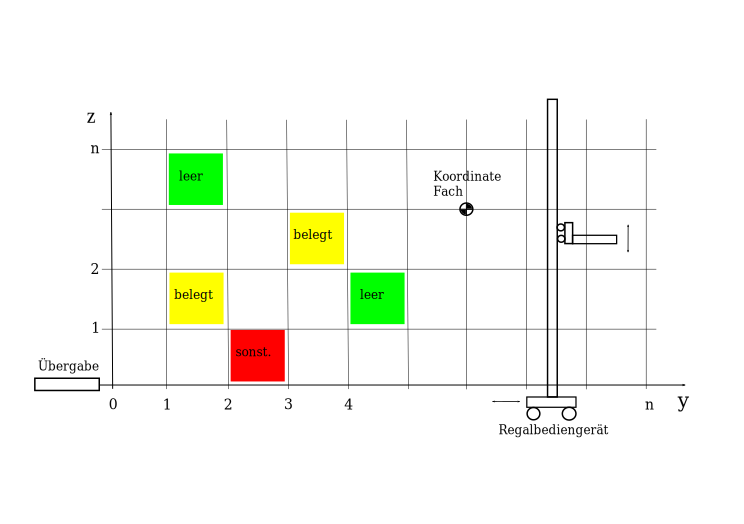
\includegraphics[width=0.9\textwidth]{images/koordinaten-wand.png}
    \caption{Lagerwand}
    \label{fig:wand}
  \end{center}
\end{figure}
%
In Abbildung \ref{fig:wand} sind ebenfalls die verwendete Farbzuordung für die Lagerplätze (Bins) ersichtlich.
%
\begin{table}
  \caption{Farbzuordung Lagerplätze}
  \label{tab:bin-color}

  \begin{center}
    \begin{tabular}{cc}
       grün & leer\\
       gelb & belegt\\
       rot & reserviert/defekt/spezial \\
    \end{tabular}
  \end{center}
\end{table}

%
\subsubsection{Klappung}
Für die zweidimensionale Darstellung wurde eine Lagergasse gemäss Abbildung \ref{fig:klapp} aufgefaltet, respektive aufgeklappt.
%
\begin{figure}[H]
  \begin{center}
    \includegraphics[width=0.7\textwidth]{images/klappung.png}
    \caption{Klappung}
    \label{fig:klapp}
  \end{center}
\end{figure}

%
\subsection{Mathematische Grundlagen}
Regalbediengerät bewegt sich zwischen den Lagerwänden auf der y- und der z-Achse. Der Arm des Regalbediengerät verfährt auf der y-Achse und der Ausleger auf der z-Achse. Die Bewegungen auf beiden Achsen lassen somit beliebige Verfahrwege auf der yz-Ebene zu. 
%
Die Grundgleichung für die Geschwidigkeit in der Ebene lautet:
%
\begin{equation}
v = \frac{s}{t}
\end{equation}
%
Die Fahrt des Regalbediengerät besteht aus einer Phase für die Beschleunigung, einer Phase der gleichförmigen Bewegung mit möglichst maximaler Geschwindigkeit und einem Bremsabschnitt, resp. einer Verzögerungsphase, am Ende. 
%
Die kürzeste Fahrzeit ergibt sich auch mehreren Faktoren. Die Synchronisationsgerade ist ein in diesem Zusammenhang oft verwendeter Begriff, welcher die optimale Fahrbahn des Regalbediengerät beschreibt. Dieser Fahrbahn führt jedoch nicht zur optimalen Fahrzeit, da unter Umständen beide Achsen gebremst werden müssten. Wir haben aber den Ansatz gewählt, dass, wenn möglich, nur auf der schnelleren Achse die Geschwindigkeit reduziert wird, was dazuführt, dass sich die zweite Achse entsprechend ihrem Maximum fortbewegen kann.
%
Ein Grenzfall tritt auf, wenn die zu bewältigende Strecke kleiner wird als die Summe der Wege von der Beschleunigung und Verzögerung bei konstanten Beschleunigungen/Verzögerungen und Geschwindigkeiten. 
%
\begin{equation}
v = \sqrt{\frac{2 \cdot s \cdot a \cdot d}{(a+d)}}
\end{equation}
%
\subsection{Simulationstechnische Grundlagen}





%EOF
